\chapter{Blockchain}

\section{Generalities}
\label{sec:ch2sec1}
A blockchain is a growing collection of items known as blocks that is stored in a decentralized, transparent, and secure ledger. Each block is linked to the previous one using hashes to form an unbreakable chain. Blockchains come are useful in a lot of scenarios where having a centralized middleman is not required. Currently, peer-to-peer currency represent the main use case for blockchain technology. cryptocurrencies that keep track of all user balances and transactions without the assistance of a single third. Bitcoin was the first blockchain of this kind as was defined as: "A purely peer-to-peer version of electronic cash would allow online payments to be sent directly from one party to another without going through a financial institution"\cite{nakamoto2008bitcoin}. The main characteristics of Bitcoin are:
\begin{itemize}
	\item Decentralisation: No sigle entity controlls the blockchain. It is managed by a distributed network of nodes.
	\item Imutability: Once a transaction is recorded on the blockchain it is almoast impossible to change it in the future
	\item Transparency: Everyone can view every transaction on the blockchain and everyones balance since the begining of the blockchain
	\item Security: Data on the blockchain is protected from modification and hacking by strong encryption.
\end{itemize}
\par With only 21 million bitcoins ever created, it is currently considered digital gold. Bitcoin was a groundbreaking idea. However, it is not without its shortcomings. Among them include the fact that Visa offers 24000 TPS whereas Bitcoin only allows 7 TPS (transactions per second). Another disadvantage is that fees are paid in Bitcoin. This meant that transactions were quite inexpensive when it initially launched, but since then, the price has increased from roughly zero to seventy thousand dollars, and fees have also increased. At the moment, a transfer costs about \$6, but this is becoming worse every day.
Because of this limitations since then over 1000 blockchains appeared according to Watcher Guru \cite{watcherguru}
\par Ethereum is the 2nd blockchain by market capitalization after bitcoin. After overcoming the early constraints of Bitcoin, the introduction of Ethereum signaled a turning point in the development of blockchain technology. Co-founder of Ethereum, Vitalik Buterin, pointed out that blockchain technology has applications beyond just transferring money. His goal was to build a programmable computer running code on top of Ethereum, a flexible framework for decentralised applications (DApps).
\par Buterin introduced the idea of a programmable blockchain with its own programming language, Solidity, for creating smart contracts in the Ethereum whitepaper, which was published in 2013. The description of Ethereum is "A Next-Generation Smart Contract and Decentralized Application Platform." \cite{ethereumwhitepaper}
\par The possibilities for blockchain are endless thanks to the capacity to write self-executing smart contracts. At its core, Ethereum is a worldwide network of nodes that can execute smart contract code thanks to the Ethereum Virtual Machine (EVM). Transaction fees or "gas" are paid for with ether money (ETH), which is also used to compensate network miners. Ethereum is now the foundation of a flourishing DApp ecosystem that is promoting innovation across many industries. The idea of Web3, which envisions a more user-based, decentralized internet, has been strengthened by it.

\section{How do cryptocurrencies work?}
\label{sec:ch2sec2}
\par Blockchain uses public and private key cryptography to ensure the security and integrity of transactions. This cryptography system is essential to the operation of blockchain technologies, including cryptocurrencies. Here's how it works:
\begin{enumerate}
	\item Key generation: A pair of cryptographic keys—a private key and a public key—are generated for every blockchain user - tipically by a crypto wallet. While the public key is open for distribution, the private key is confidential and needs to be kept secure by the user. Although there is a mathematical relationship between these keys, the private key cannot be obtained from the public key. With the public key a unique address is generated.
	\item Transaction creation: When a user wants to initiate a transaction, for example, send tokens to another account, they create a transaction message. This message includes information such as the recipient's address, the amount transferred and other optional data.
	\item Signing the transaction: With their private key, the user signs the transaction. Each transaction generates a unique digital signature using the private key, which acts as mathematical evidence that the person whose private key is linked to the account from which the money is being transferred approved the transaction.
	\item Transaction Verification: Using the sender's public key, the network's nodes—or miners, in the case of Bitcoin—verify the transaction's digital signature after it has been published on the blockchain. The transaction is regarded as authentic and can be completed if the signature is legitimate.
	\item At last, the transaction is added to the blockchain by being included in a new block that is subsequently appended to the current chain of blocks upon validation—thus the term "blockchain." The transaction becomes permanent and irrevocable once it is recorded to the blockchain, offering a transparent and safe record of the money transfer.
\end{enumerate}
\begin{figure}[htbp]
	\centering
	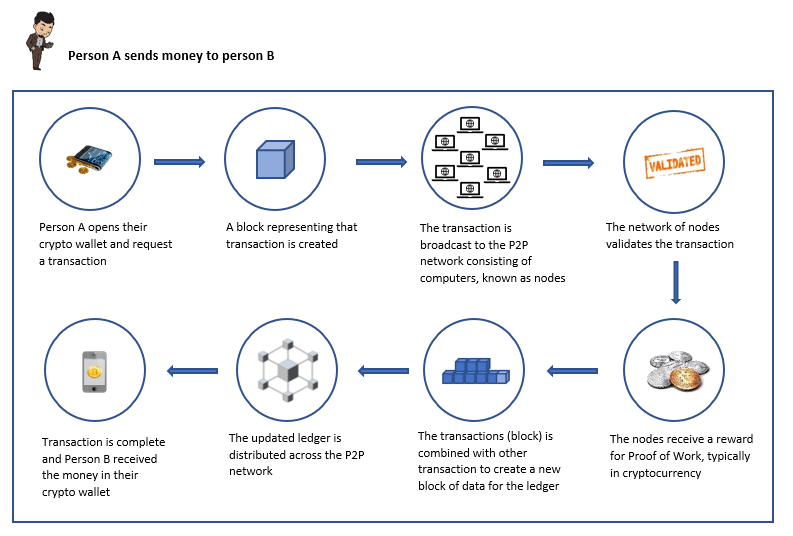
\includegraphics[scale=1]{./figures/crypto-flow.png}
	\caption{Sending a transaction flow}
\end{figure}
\par Blockchain utilizes cryptography in these ways to offer a decentralized, transparent, and extremely safe payment system without the need for a dependable central authority like a bank or other financial middleman.

\section{Smart Contracts}
\label{sec:ch2sec3}
For a person that has not much experience with blockchain development, smart contracts are functions that are deployed on the blockchain and can be called by everyone. After the deployment the smart contract code cannot be altered. Investopidia defines smart contracts as: "a self-executing program that automates the actions required in an agreement or contract. Once completed, the transactions are trackable and irreversible. Smart contracts permit trusted transactions and agreements to be carried out among disparate, anonymous parties without the need for a central authority, legal system, or external enforcement mechanism"\cite{smartcontracts}. Some applications of smart contracts are the following:

Decentralized Finance (DeFi):
\begin{itemize}
	\item Liquid Staking: Users can stake their ETH on websites like as Lido or Rocket Pool, and in exchange, they will obtain liquid tokens equivalent to their ETH worth. Then, by using these liquid tokens in different DeFi protocols, more returns can be produced.
	\item Descentralized exchanges: Users can exchange various crypto-assets directly with one another without the necessity of centralized middlemen thanks to decentralized exchanges (DEX) like Uniswap and SushiSwap
	\item Lending and borrowing: Users can deposit or lend cryptocurrency assets to earn interest through platforms like Aave or Compound. All transactions are openly managed by smart contracts.
\end{itemize}

NFT Markets: Using smart contracts, marketplaces such as OpenSea or Rarible enable the buying, selling, and trade of unique tokens (NFTs), which stand in for digital art pieces, collectibles, or game assets.

 Decentralized autonomous organizations (DAO), such as MakerDAO, use smart contracts to enable token holders to speak up for themselves and cast votes on decisions that will determine the protocol's future development.
 
 Blockchain gaming: Smart contracts facilitate the management of game economies, include NFT components into the game, and guarantee a fair and transparent game for all players.
 
 \section{Crypto Wallets}
 \label{sec:ch2sec4}
\par  Cryptocurrency wallets are digital tools that allow users to store and manage their cryptographic keys used to transact with cryptocurrencies such as Bitcoin, Ethereum, and others. These wallets can exist in various forms, from software applications to hardware devices, and are essential for using cryptocurrencies in a safe and efficient way. Shortly put, a crypto wallet hold one or more private key for you to interact with the blockchain.
\par Wallets for cryptocurrencies serve a number of crucial purposes:
\begin{itemize}
	\item Security: Offers a safe space to save private keys, which are necessary to when using cryptocurrencies, because whoever access the private key has full access to the funds.
	\item Interacting with the blockchain: Make it possible to send and receive money using cryptocurrencies, enabling transfers, or DApps interactions.
	\item Interoperability: Enables users to engage with many blockchains and take part in multiple ecosystems such as Bitcoins, Ethereum etc.
	\item Control: Gives users complete control over their digital assets without the need for intermediaries such as banks.
\end{itemize}
\par Cryptocurrency wallets fall into several categories, depending on the nature and level of security offered:
\begin{enumerate}
	\item Software wallets: These are computer or mobile applications that can be downloaded. Although they are practical, their degree of security is dependent on how secure the host device is. For instance, if your computer is compromised by malware or viruses and you have an extension wallet, the private key could be taken.
	\item Hardware wallets: These are physical devices that store and generate private keys offline, providing increased security. The private key is also stored on a hardware device and it never leaves it. They are considered some of the safest options for long-term cryptocurrency storage.
	\item Paper wallets: Involves printing private and public keys on paper, which are then stored in a secure location. They eliminate the risks associated with cyber attacks, but are susceptible to physical risks such as damage or loss. Almost every time a hardware wallet will be better than this.
\end{enumerate}

To enable access to and trade of cryptocurrencies, private key wallets employ pairs of private and public keys. They offer a high level of security as long as the private key is safeguarded and kept secret, and they are simple to use and the foundation of the majority of bitcoin wallets currently in use.

However, smart contract wallets handle transactions using smart contracts on Ethereum and other platforms. Advanced capabilities that these wallets can offer include approving transactions from several parties at once or incorporating intricate trade rules straight into the contract logic. Smart contract wallets are perfect for sophisticated usage, such as automatically managed money or wallets that need several approvals to conduct a transaction, because of their considerable customization and automation options. Even if smart contracts wallets are much more sophisticated, to interact with them you still need to use a wallet with a private key, however, they can add features to increase security.

 \section{Multisignature Wallets}
\label{sec:ch2sec5} 
Multisig wallets, sometimes referred to as multi-signature wallets, are an important development in the security of cryptocurrencies. They improve the security of monies that are kept in storage by requiring the consent of several parties before executing a transaction.

A smart contract that specifies how many of the preset holders must sign a transaction before it is performed is the foundation of a multisig wallet. A wallet can be set up, for instance, so that two of the three holders must sign it. This system strikes a balance between security and accessibility by preventing illegal acts and preventing the loss of access to funds in the event that a single key is compromised.
\begin{figure}[htbp]
	\centering
	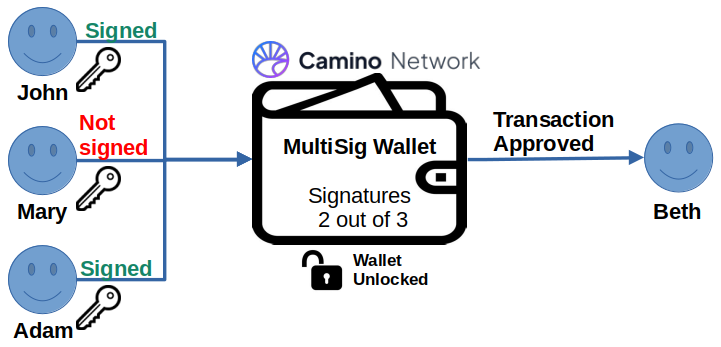
\includegraphics[scale=0.65]{./figures/multisig-flow.png}
	\caption{Approving a transaction with a multisig wallet}
\end{figure}


Comparing multisig wallets to conventional single-signature wallets reveals numerous noteworthy benefits. The most important thing is more security. The possibility of theft or fraudulent transactions is significantly decreased by needing numerous permissions. Multisig wallets are perfect for groups or organizations that manage shared assets since they also make it easier for members to collaborate and manage funds together.

 \section{Account Abstraction}
\label{sec:ch2sec6} 
Account Abstraction is an emerging concept in the Ethereum ecosystem that promises to bring a new level of flexibility and security to blockchain users. Essentially, Account Abstraction allows users to define their account logic in a more complex and customized way, using smart contracts instead of traditional private key accounts. This approach opens the door to a number of advanced functionalities not possible with standard accounts.

Account Abstraction in the context of Ethereum allows users to use smart contracts to manage and control their accounts. Basically, the account itself becomes a smart contract that can have complex rules and conditions for making transactions. This brings several advantages, including advanced security, flexibility and customization, key recovery and automation.

\textbf{Advanced Security:} An abstracted account may include additional security mechanisms such as multi-factor authentication or limiting transactions based on various criteria (eg daily spending limits). This reduces the risk of unauthorized access and theft.

\textbf{Flexibility and Customization:} Users can define specific logic for their transactions. For example, accounts can be created that require multi-party approval (multisig) or that automatically perform certain actions based on predefined conditions.

\textbf{Key Recovery:} If a private key is lost, Account Abstraction allows the implementation of access recovery mechanisms. These mechanisms may include approval by other trusted users or the use of alternative authentication methods.

\textbf{Automation and Programmability:} Smart contracts can automate many aspects of fund management, such as recurring payments, automatic distribution of funds, or integration with other blockchain services.

To implement Account Abstraction in Solidity, developers create smart contracts that define account logic. These contracts may include functions for initiating transactions, verifying multiple signatures, and enforcing security rules.

For example, a simple contract in Solidity for an abstracted account would include an owner, a set of guardians who can approve transactions, and a function to execute transactions after they are approved by a sufficient number of guardians. This type of contract allows for increased security and customization, adapting to the individual needs of users.

Account Abstraction represents a major step forward in the evolution of blockchain technology, giving users and developers the tools to create more secure, flexible and innovative solutions. As standards and solutions for this technology continue to develop, we can expect a wider integration of abstracted accounts into the Ethereum ecosystem, which will lead to increased security and a more efficient and personalized use of digital funds.

 \section{Ethereum Virtual Machine and Layer 2s}
\label{sec:ch2sec7} 
The Ethereum Virtual Machine (EVM) is the central engine that enables smart contracts to run on the Ethereum blockchain. EVM is a Turing-complete runtime, meaning it can execute any computational logic defined by smart contract code. Each node in the network runs EVM, ensuring that transactions are executed in a consistent and verifiable manner. Smart contracts are written in Solidity, a contract-oriented programming language that compiles and can be deployed on any EVM-compatible chain.

As Ethereum has grown in popularity, the network has faced significant scalability and cost challenges. Transactions on Ethereum can become slow and expensive during periods of high demand due to limited transaction processing capacity. To address these issues, Layer 2 solutions have been developed, which run on top of the main Ethereum network (Layer 1) and allow for increased transaction capacity without sacrificing security or decentralization.

Optimism and Arbitrum are one of the most prominet Layer 2 solutions developed to improve Ethereum scalability.

\section{Optimism}
Optimism is a Layer 2 solution based on Optimistic Rollup technology. This allows the execution of smart contracts on a secondary layer, aggregating multiple transactions into a single transaction on the main layer. Transactions are considered valid by default (optimistic), with the possibility of being challenged in case of fraudulent activity.

\textbf{How Optimism works:}

Transaction Aggregation: Transactions are grouped and processed on the secondary layer. This significantly reduces the number of transactions that need to be processed on the core layer.
Fraud-Proof Verification: Because transactions are considered valid by default, there is a period of time in which they can be disputed by other nodes. If fraud is discovered, the transaction is voided.
Low Fees: Due to the reduction in the number of transactions that need to be processed on the main layer, transaction costs are much lower compared to Ethereum. Optimism fees are usually a fraction of the main layer fees, often around 1/10th or less.
Block Time: The block time on Optimism is much faster than on Ethereum, facilitating fast and efficient transactions.

\section{Arbitrum}
Arbitrum is another Layer 2 solution that uses Optimistic Rollup technology to improve Ethereum's scalability and efficiency. Arbitrum offers full EVM support, meaning that smart contracts written in Solidity can be implemented on Arbitrum without major modifications. This facilitates the adoption of Arbitrum by developers and users who are already familiar with the Ethereum ecosystem.

\textbf{How Arbitrum works:}

Transaction Aggregation: Similar to Optimism, Arbitrum aggregates multiple transactions into a single transaction that is processed on the Ethereum core layer.
Validation and Dispute: Transactions are considered valid by default, but can be disputed within a specified period. If a transaction is disputed and found to be fraudulent, it is invalidated.
Low Fees: Arbitrum offers transactions with much lower fees compared to Ethereum main layer. The fees on Arbitrum are usually similar or even lower than those on Optimism.
Block Time: Arbitrum has a very fast block times, under 1 seconds, at the moment is the faster layer 2 present.

These Layer 2 solutions play a crucial role in improving the performance of Ethereum, facilitating the widespread adoption of blockchain technology by providing fast and cheap transactions while maintaining the security and decentralization of the network.